\section{Introduction to \code{if}-Expressions}
In this section, we'll discuss how to implement \code{if}-expressions. Our concrete syntax for this extension will look like 
\begin{verbatim}
(*
    expr :=
        | <number>
        | true                              // New!
        | false                             // New!
        | <name>
        | (add1 <expr>)
        | (sub1 <expr>)
        | (+ <expr> <expr>)
        | (let (<name> <expr>) <expr>)
        | (if <expr> <expr> <expr>)         // New!
        | ... 
*)\end{verbatim}

\subsection{Structure of \code{if}-Expressions}
An \code{if}-expression looks like 
\begin{verbatim}
    (if <expr> <expr> <expr>)\end{verbatim}

\begin{itemize}
    \item Here, the first \code{<expr>} represents the condition expression; this determines which of the subsequent expressions should be executed. 
    \item The second \code{<expr>} represents the ``then'' expression; this expression should be executed if the condition expression resolves to \code{true}.
    \item The third and last \code{<expr>} represents the ``else'' expression; this expression should be executed if the condition expression resolves to \code{false}.
\end{itemize}
Before we talk more about how \code{if}-expressions should be evaluated, we need to figure out how \code{if}-expressions should work in the first place in terms of what is allowed and what isn't. 

\subsection{Boolean Values}
Let's begin by figuring out what some sample programs should resolve to.
\begin{mdframed}
    (Exercise.) What should the following programs evaluate to? 
    \begin{enumerate}[a.]
        \item \begin{verbatim}
(let (x 5)
    (if (= x 10) (+ x 2) x))\end{verbatim}

        \begin{mdframed}
            This should evaluate to \code{5}. We first defined $x = 5$ and then used that in our \code{if}-expression to see if $x = 10$; since it doesn't, we just return \code{x}, which is 5.  
        \end{mdframed}


        \item \begin{verbatim}
(if 5 true false)\end{verbatim}

        \begin{mdframed}
            There are several reasonable answers we can consider here. 
            \begin{itemize}
                \item \code{true}: since \code{5} is a truthy value (i.e., evaluates as a true expression), it would make sense for this program to return \code{true}.
                \item \code{false}: since \code{5} isn't a boolean expression, we could just have the program return \code{false}.
                \item an error: since \code{5} isn't a boolean expression, we can throw an error telling the user that this isn't an boolean expression. 
            \end{itemize}
            In our class, we'll say \code{true}. In other words, we're allowing truthy and falsy values.
        \end{mdframed}


        \item \begin{verbatim}
(+ 7 true)\end{verbatim}

        \begin{mdframed}
            There are two answers we can have for this. 
            \begin{itemize}
                \item \code{8}: if \code{true} implicitly resolves to \code{1}, then this is just $7 + 1 = 8$.
                \item an error: since \code{7} and \code{true} are different types, it wouldn't make sense to add them. 
            \end{itemize}
            In our class, we'll say that this expression should throw an error at compile-time.
        \end{mdframed}

        \item \begin{verbatim}
(= true 1)\end{verbatim}

        \begin{mdframed}
            There are two answers we can have for this. 
            \begin{itemize}
                \item \code{true}: for the same reason as above.
                \item an error: for the same reason as above. 
            \end{itemize}
            In our class, we'll say that this expression should throw an error at compile-time.
        \end{mdframed}
    \end{enumerate}
\end{mdframed}
Based on our discussion above, in this class, 
\begin{itemize}
    \item We'll allow truthy and falsy values to be resolved to boolean types (\code{true} and \code{false}, respectively) when used as conditions in \code{if}-expressions.
    \item We won't allow the mixing of types when doing comparison (e.g., \code{=}, \code{<}, etc.) or arithmetic (e.g., \code{+}, \code{-}) operations. These should throw an error during runtime\footnote{In our class, we won't be working on a type checker. However, if we did work on a type checker, then we could make mixing of types when doing these operations a compile-time (parse) error.}.
\end{itemize}

\subsection{Boolean Representation}
With the above discussion in mind, how should we best represent boolean values in assembly?

\begin{mdframed}
    (Exercise.) \emph{Intuitively} (i.e., using our knowledge from previous sections), what should be in \code{RAX} after these are done evaluating? 

    \begin{enumerate}[a.]
        \item \code{1}
        \begin{mdframed}
            Trivially, we just move \code{1} into \code{RAX}.
        \end{mdframed}

        \item \code{5}
        \begin{mdframed}
            Trivially, we just move \code{5} into \code{RAX}.
        \end{mdframed}

        \item \code{-3}
        \begin{mdframed}
            Trivially, we just move \code{-3} into \code{RAX}.
        \end{mdframed}

        \item \code{true}
        \begin{mdframed}
            There's not exactly a way to directly represent \code{true} in assembly, so the best we can do is a truthy value. For now, let's just move \code{1} into \code{RAX}.
        \end{mdframed}

        \item \code{false}
        \begin{mdframed}
            Same idea as before: the best we can do is a falsy value. For now, let's just move \code{0} into \code{RAX}.
        \end{mdframed}

        \item \code{(= 3 5)}
        \begin{mdframed}
            Since $3 = 5$ is false, we can just put \code{0} into \code{RAX}.
        \end{mdframed}

        \item \code{(+ 4 7)}
        \begin{mdframed}
            Trivially, we just move the result of $4 + 7$, or \code{11}, into \code{RAX}.
        \end{mdframed}
    \end{enumerate}
\end{mdframed}
Remember that we didn't want the mixing of types when doing any comparison or arithmetic operations, e.g., \code{(+ 5 true)} should throw an error. However, with our answers above, how do we know that the \code{1} in \code{RAX} isn't actually a \code{true} value? 

\subsection{A New Representation of Numbers: Tagging}
We will now represent numbers as \textbf{64-bits} instead of 32-bits like in previous sections. With this in mind, this is 64 bits:
\begin{verbatim}
    0000 0000 0000 0000 0000 0000 0000 0000 0000 0000 0000 0000 0000 0000 0000 0000\end{verbatim}
The number 5 can be represented like so: 
\begin{verbatim}
    0000 0000 0000 0000 0000 0000 0000 0000 0000 0000 0000 0000 0000 0000 0000 0101\end{verbatim}

Let's suppose we \emph{shift} 5 one to the left to get the number 10: 
\begin{verbatim}
    0000 0000 0000 0000 0000 0000 0000 0000 0000 0000 0000 0000 0000 0000 0000 1010\end{verbatim}

If we're okay with 63-bit numbers, we can use the \textbf{least significant bit} (i.e., the right-most bit) as a \textbf{tag}. This tag tells us if the value is a number or a boolean value. In this class, 
\begin{itemize}
    \item Numbers will have a least significant bit of \code{0}.
    \item Booleans will have a least significant bit of \code{1}. 
\end{itemize}
For example, we can represent the number \code{13} as 
\begin{verbatim}
    0000 0000 0000 0000 0000 0000 0000 0000 0000 0000 0000 0000 0000 0000 0001 1010\end{verbatim}
We can represent the boolean \code{false} as 
\begin{verbatim}
    0000 0000 0000 0000 0000 0000 0000 0000 0000 0000 0000 0000 0000 0000 0000 0001\end{verbatim}
We can represent the boolean \code{true} as 
\begin{verbatim}
    0000 0000 0000 0000 0000 0000 0000 0000 0000 0000 0000 0000 0000 0000 0000 0011\end{verbatim}
We can represent the number \code{0} as 
\begin{verbatim}
    0000 0000 0000 0000 0000 0000 0000 0000 0000 0000 0000 0000 0000 0000 0000 0000\end{verbatim}
    
\subsection{Consequences of Tagging}
Because we effectively have to shift everything one to the left to introduce tagging, we need to think about a few things.
\begin{itemize}
    \item \underline{\textbf{Addition}}
    \begin{itemize}
        \item When we are performing any binary (or unary) operations, we need to check if the least significant bit is correct for the given input. For example, when we are doing addition, we should check if the least significant bit of both inputs are \code{0} (implying that both are numbers). If any one of them isn't, then we should throw an error.
        \item Otherwise, addition is pretty straightforward. Assuming we have two numbers, adding two numbers should not change since the addition of both least significant bits will be 0 (since $0 + 0 = 0$). In other words, something like \code{(+ 3 5)} will generate the assembly 
        \begin{verbatim}
    mov rax, 6              ; 3 / 11 (decimal / binary)  
                            ; -> 6 /   110 (decimal / binary) accounting for tag
    mov [rsp - 16], rax 
    mov rax, 10             ; 5 / 101 (decimal / binary) 
                            ; -> 10 / 1010 (decimal / binary) accounting for tag 
    add rax, [rsp - 16]     ; 6 + 10 -> 10000 (with tagging)\end{verbatim}
        Notice how \code{10000} in binary is \code{16} in decimal. However, if we shift this answer by one to the \emph{right}, we get \code{8}, the answer to $3 + 5$.
    \end{itemize}
    \item \underline{\textbf{Multiplication}}
    \begin{itemize}
        \item Multiplication is similar to addition, except we want to make sure we shift one of the two inputs by 1 to the right before we perform the actual multiplication. So, \code{(* 3 5)} should produce the assembly
        \begin{verbatim}
            mov rax, 6              ; 3 ->  1100 accounting for tag
            mov [rsp - 16], rax 
            mov rax, 10             ; 10 -> 1010 accounting for tag
            sar rax, 1              ; 5  ->  101 (remove tagging)
            imul rax, [rsp - 16]    ; 6 * 5 -> 11110000\end{verbatim}
        \code{11110} in binary is \code{30} in decimal. Shifting this by 1 to the right gives us the desired answer of \code{15}. The reason why we choose to shift one of the two values to the right by 1 is so we can avoid potential overflow errors.
    \end{itemize}

    \item \underline{\textbf{Errors}}
    \begin{itemize}
        \item If we get an error (e.g., a type mismatch error), then from our assembly code, we want to call a \emph{Rust} function that handles the error. 
        \item For example, we might have something like 
        \begin{verbatim}
            and rax, 1 
            cmp rax, 1      ; if we get a boolean value instead of number
            je error_label  ; jump to the error_label error 
                            ; otherwise, fall through label
            ...
        error_label: 
            call rust_error\end{verbatim}
        with corresponding Rust code 
        \begin{verbatim}
            fn error() {
                panic!("error");
            }\end{verbatim}
    \end{itemize}
\end{itemize}


\subsection{Assembly Review}
There are some new assembly commands to know.
\begin{itemize}
    \item \code{cmp <reg>, <val>}: computes \code{<reg> - <val>} and sets the appropriate condition codes\footnote{The only ones that matter to us are Overflow, Sign, and Zero}. This does not modify \code{<reg>}.
    \item \code{<label>:  }: Sets this line as a label for jumping to later. 
    \item \code{and <reg>, <value>}: Performs bitwise AND on \code{<reg>} and \code{<value>}. 
    \item \code{jmp <label>}: Unconditionally jumps to \code{<label>}.
    \item \code{jne <label>}: Jumps to \code{<label>} if Zero is not set (last \code{cmp}ed values not equal).
    \item \code{je <label>}: Jumps to \code{<label>} if Zero is set (last \code{cmp}ed values equal).
    \item \code{jge <label>}: Jumps to \code{<label>} if Overflow is the same as Sign (corresponds to \code{>=} for last \code{cmp}).
    \item \code{jle <label>}: Jumps to \code{<label>} if Zero is set or Overflow is not equal to Sign (corresponds to \code{<=} for last \code{cmp}).
    \item \code{shl <reg>}: Shifts \code{<reg>} to the left by 1, filling in least-significant bit with zero.
    \item \code{sar <reg>}: Shifts \code{<reg>} to the right by 1, filling in most-significant bit to preserve sign
    \item \code{shr <reg>}: Shifts \code{<reg>} to the right by 1, filling in most-significant bit with zero.
\end{itemize}

\subsection{Modifying the Runtime}
In our class, we had a \code{runtime.rs} file which was responsible for calling our assembly code and printing out the result; this looks something like:
\begin{verbatim}
    #[link(name = "our_code")]
    extern "C" {
        #[link_name = "\x01our_code_starts_here"]
        fn our_code_starts_here() -> i64;
    }
    
    fn main() {
        let i: i64 = unsafe { our_code_starts_here() };
        println!("{i}");
    }\end{verbatim}
One thing to consider here is that, with our new tagging system, we have two problems
\begin{itemize}
    \item The code above won't print out boolean values properly (it'll either print out \code{3} or \code{1}, not \code{true} or \code{false} like we would hope).
    \item It also won't print out the numbers correctly. Remember that the integers have been shifted one bit to the left, and this code doesn't account for that when printing the result. So, if the code is supposed to print \code{5}, then this would actually print \code{10}. 
\end{itemize}
The solution is to modify this file so that it can correctly interpret the resulting value that the assembly code produces. We might have something like the below.
\begin{verbatim}
    fn main() {
        let i: i64 = unsafe { our_code_starts_here() };
        // If we have an integer (remember that, for numbers, the LSB should be 0)
        if i & 1 == 0 {
            println!("{}", i >> 1);
            return;
        }

        // Otherwise, i & 1 -> 1, so we should have a boolean value. Let b 
        // be either 0 or 1 (if we have a valid boolean).
        let b = i >> 1;
        // If b is 0 or 1, then we have a boolean value.
        if b == 0 || b == 1 {
            println!("{}", b == 1);
        } else {
            println!("unknown value: {i}");
        }
    }\end{verbatim}

\subsection{The Abstract Syntax}
Recall that an \code{if}-expression looks something like 
\begin{verbatim}
    (if <expr> <expr> <expr>)\end{verbatim}
where 
\begin{itemize}
    \item the first \code{<expr>} represents the condition expression; this determines which of the subsequent expressions should be executed. 
    \item the second \code{<expr>} represents the ``then'' expression; this expression should be executed if the condition expression resolves to \code{true}.
    \item the third and last \code{<expr>} represents the ``else'' expression; this expression should be executed if the condition expression resolves to \code{false}.
\end{itemize}
As defined in the grammar, we also need to be able to support boolean values (\code{true} and \code{false}). This is trivially just \code{True} and \code{False} in the abstract syntax. So, the abstract syntax will look like 
\begin{verbatim}
    enum Expr {
        Num(i32),
        True,                                   // New!
        False,                                  // New!
        Add1(Box<Expr>),
        Plus(Box<Expr>, Box<Expr>),
        Let(String, Box<Expr>, Box<Expr>),
        Id(String),
        Eq(Box<Expr>, Box<Expr>),               // New!
        If(Box<Expr>, Box<Expr>, Box<Expr>)     // New!
    }\end{verbatim}

\subsection{Extending the Parser}
Because our \code{if}-expression is basically a list of four expressions, we just need to match that particular pattern. So, parsing \code{if}-expressions should be straightforward. 
\begin{verbatim}
    match s {
        ...
        Sexp::List(list) => match &list[..] {
            [Sexp::Atom(S(keyword)), cond, thn, els] if keyword == "if" => Expr::If(
                Box::new(parse_expr(cond)),
                Box::new(parse_expr(thn)),
                Box::new(parse_expr(els)),
            )
            ...    
        }
    }\end{verbatim}
So, how do we represent boolean types? One way is by looking at the identifier: if the identifier happens to be \code{true} or \code{false}, we can assume that this is a \code{boolean} type. Otherwise, we can assume that we just have a regular identifier.
\begin{verbatim}
    match s {
        Sexp::Atom(S(id)) => {
            if id == "true" {
                Expr::True
            } else if id == "false" {
                Expr::False
            } else {
                Expr::Id(id.to_owned())
            }
        }
        ...
    }\end{verbatim}
Finally, parsing the equality operator (e.g., \code{(= 10 5)}) is the same as with parsing the plus operator.

\subsection{Implementing the Compiler}
Before we start, one adjustment we need to make to account for the tagging system that we've discussed is to shift integers one bit to the left. That is, when we have an integer, we need to shift it one bit to the left so the least significant bit can be used as the tag bit.
\begin{verbatim}
    match e {
        Expr::Num(n) => format!("mov rax, {}", *n << 1),
        ... 
    }\end{verbatim}
Now, let's think about \code{if}-expressions. \code{if}-expressions imply that only a subset of code will be executed. For example, if we have an \code{if}-statement and the condition resolves to \code{false}, the code inside the \code{if}-statement will not be executed. In assembly, we can represent this behavior using \textbf{branches}. Roughly speaking, the assembly will look like
\begin{verbatim}
        cmp value, 3        ; if value == true {
        jne else_block      ;       // your code
        // code here        ;       // here 
        jmp done_block      ; 
    else_block:             ; } else {
        // code here        ;       // your code here
    done_block:             ; }
\end{verbatim}
What's going on?  
\begin{center}
    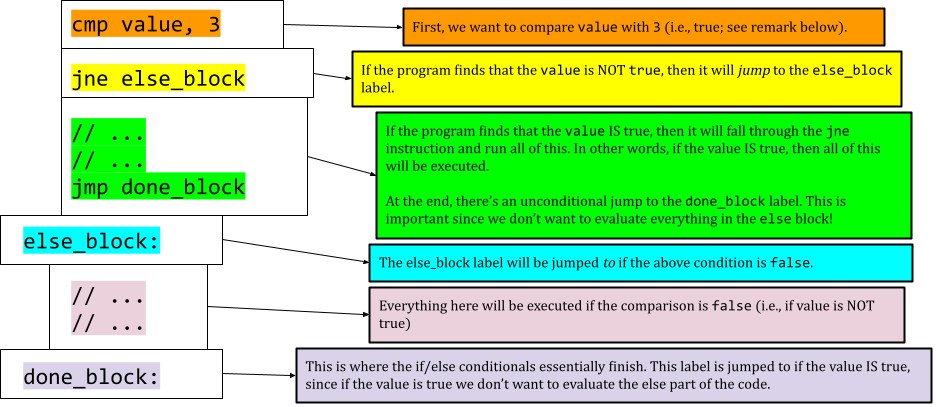
\includegraphics[scale=0.5]{assets/asm_if.png}
\end{center}
\textbf{Remark:} \code{3} is represented as \code{true} (the binary representation of \code{3} is \code{11}; notice how the tag bit is \code{1}).

\subsubsection{Duplicate Labels}

All \code{if}-expressions will follow the same pattern\footnote{Maybe not the exact pattern, but the same behavior}. However, if we just use this same exact template, we'll end up with multiple duplicate label declarations. In other words, we might end up with something like 
\begin{verbatim}
    cmp value 3
    jne else_block 
    // ... 
    jmp done_block 
else_block:
    // ... 
done_block:
    // ...
    cmp value 3
    jne else_block 
    // ... 
    jmp done_block 
else_block:
    // ... 
done_block:\end{verbatim}
This code would fail to run since there are, for example, duplicate \code{done\_block} label declarations. So, we need to create a unique label whenever we do declare a label. Let's declare a function that does just this: 
\begin{verbatim}
    fn new_label(l: &mut i32, s: &str) -> String {
        let current = *l;
        *l += 1;
        format!("{s}_{current}")
    }\end{verbatim}
At a high level, \code{new\_label} takes in a mutable reference to an integer and a string, and creates a label using those inputs. The integer is incremented -- this is important since this guarantees that every label created from this function will be unique.

\subsubsection{The Equals Comparison Operator}
How do we check if two expressions are equal? The process is relatively similar to adding two expressions. The only difference is at the end, when instead of actually \emph{adding} the values, we put either 3 (\code{true}) or 1 (\code{false}) into \code{rax}.

\bigskip 

The way we do this (putting either \code{3} or \code{1} into \code{rax}) is literally just another \code{if}-statement! At a high level, this might look like: 
\begin{verbatim}
    if rax == [rsp - stack_offset] {
        rax = 3
    } else {
        rax = 1
    }\end{verbatim}
So, compilation might look something like this: 
\begin{verbatim}
    match e {
        Expr::Eq(a, b) => {
            let a_instr = compile_expr(a, si, env, counter);
            let b_instr = compile_expr(b, si + 1, env, counter);
            let else_label = new_label(counter, "ifelse");
            let end_label = new_label(counter, "ifend");
            let stack_offset = si * 8;

            format!("
            {a_instr}
            mov [rsp - {stack_offset}], rax
            {b_instr}
            cmp rax, [rsp - {stack_offset}]
            jne {else_label}
              mov rax, 3
              jmp {end_label}
            {else_label}:
              mov rax, 1
            {end_label}:
            ")
        }
        ...
    }\end{verbatim}

\subsubsection{\code{if}-Expressions}
With everything in mind, our final implementation of \code{if}-expressions will look something like the below.
\begin{verbatim}
    match e {
        Expr::If(cond, thn, els) => {
            let end_label = new_label(counter, "ifend");
            let else_label = new_label(counter, "ifelse");
            let cond_instrs = compile_expr(cond, si, env, counter);
            let thn_instrs = compile_expr(thn, si, env, counter);
            let els_instrs = compile_expr(els, si, env, counter);
            format!(
                "
               {cond_instrs}
               cmp rax, 3
               jne {else_label}
                 {thn_instrs}
                 jmp {end_label}
               {else_label}:
                 {els_instrs}
               {end_label}:"
            )
        }
        ... 
    }\end{verbatim}
At a high level, 
\begin{itemize}
    \item First, we should evaluate the conditional part of the \code{if}-statement. We should\footnote{We'll talk more about type validation later.} end up with a boolean value in \code{rax}. 
    \item With the boolean value in \code{rax}, we can determine which code (either the ``then'' or ``else'' blocks) to run. 
\end{itemize}